\begin{frame}{A Theory of Onset Temperature in 2D: The Kosterlitz-Thouless Transition}

\begin{columns}[T]
\begin{column}[T]{0.5\textwidth}

\begin{block}{\centering \large Internal Degrees of Freedom}
Excitations have rotation + stretching modes
\end{block}

\begin{figure}
\begin{overprint}
\onslide<2>\centering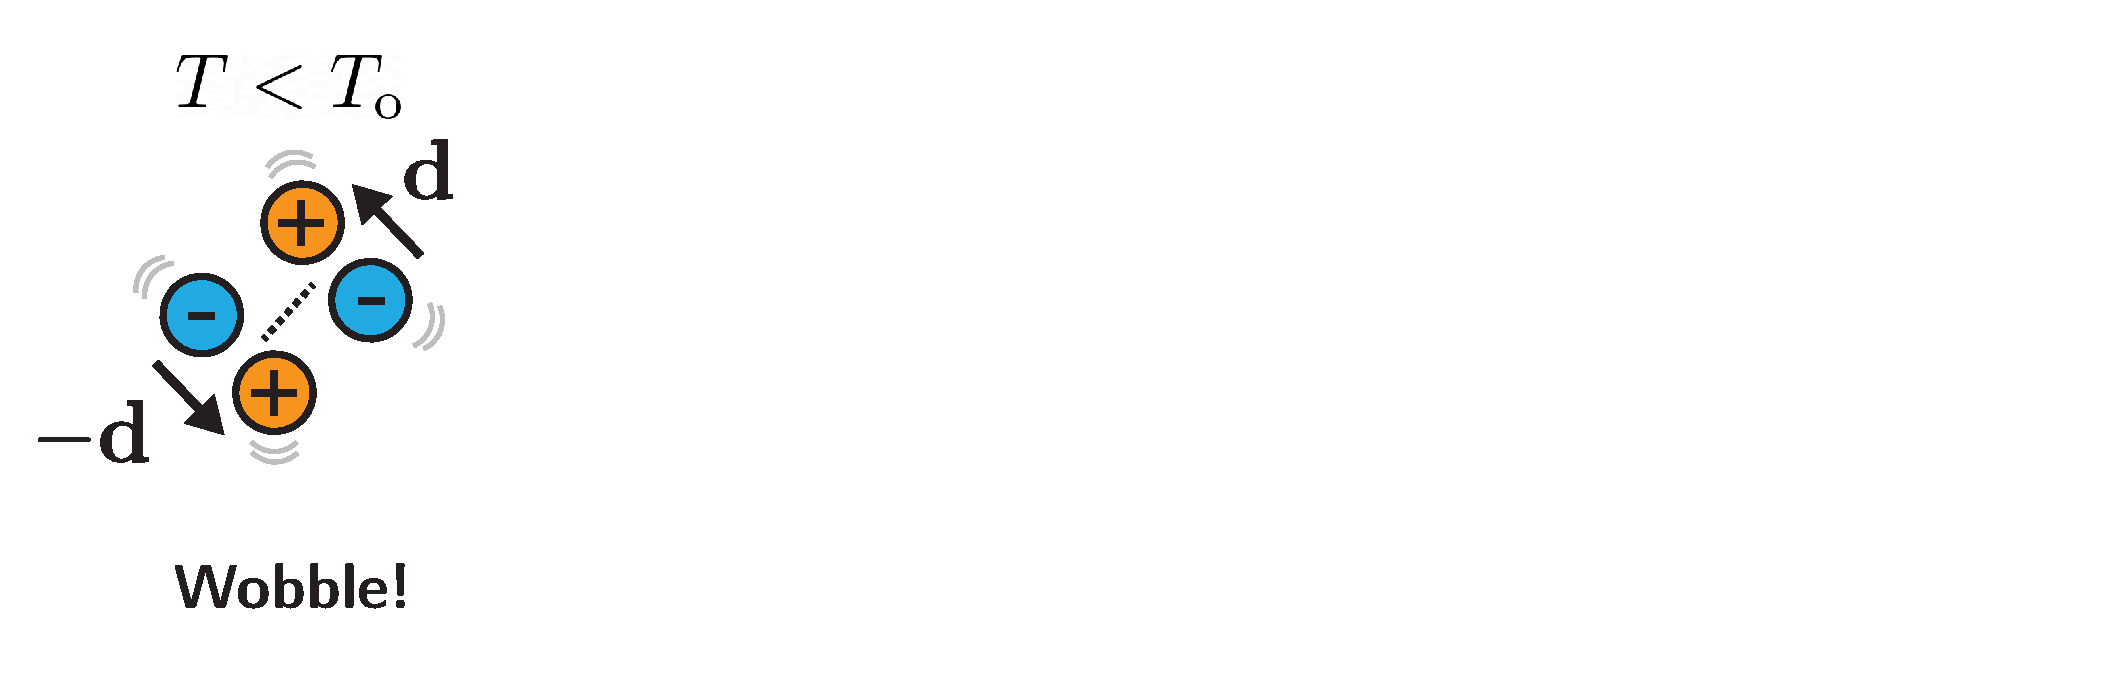
\includegraphics[width=0.85\linewidth]{c.6-kt_energyentropy/dofs_quadrupole-0.pdf}
\onslide<3>\centering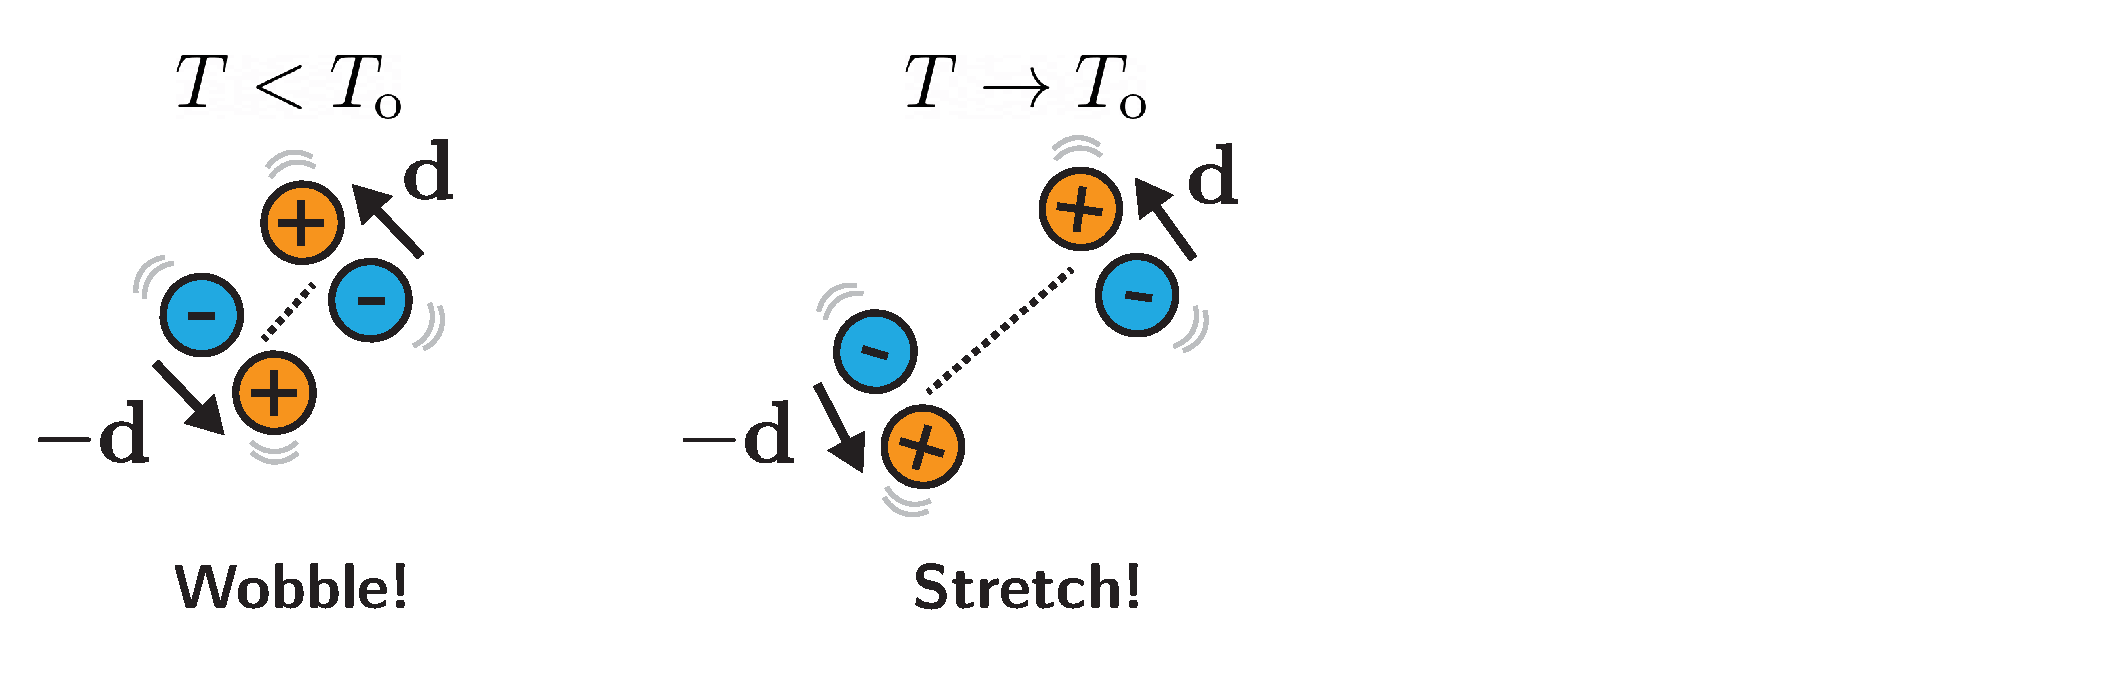
\includegraphics[width=0.85\linewidth]{c.6-kt_energyentropy/dofs_quadrupole-1.pdf}
\onslide<4->\centering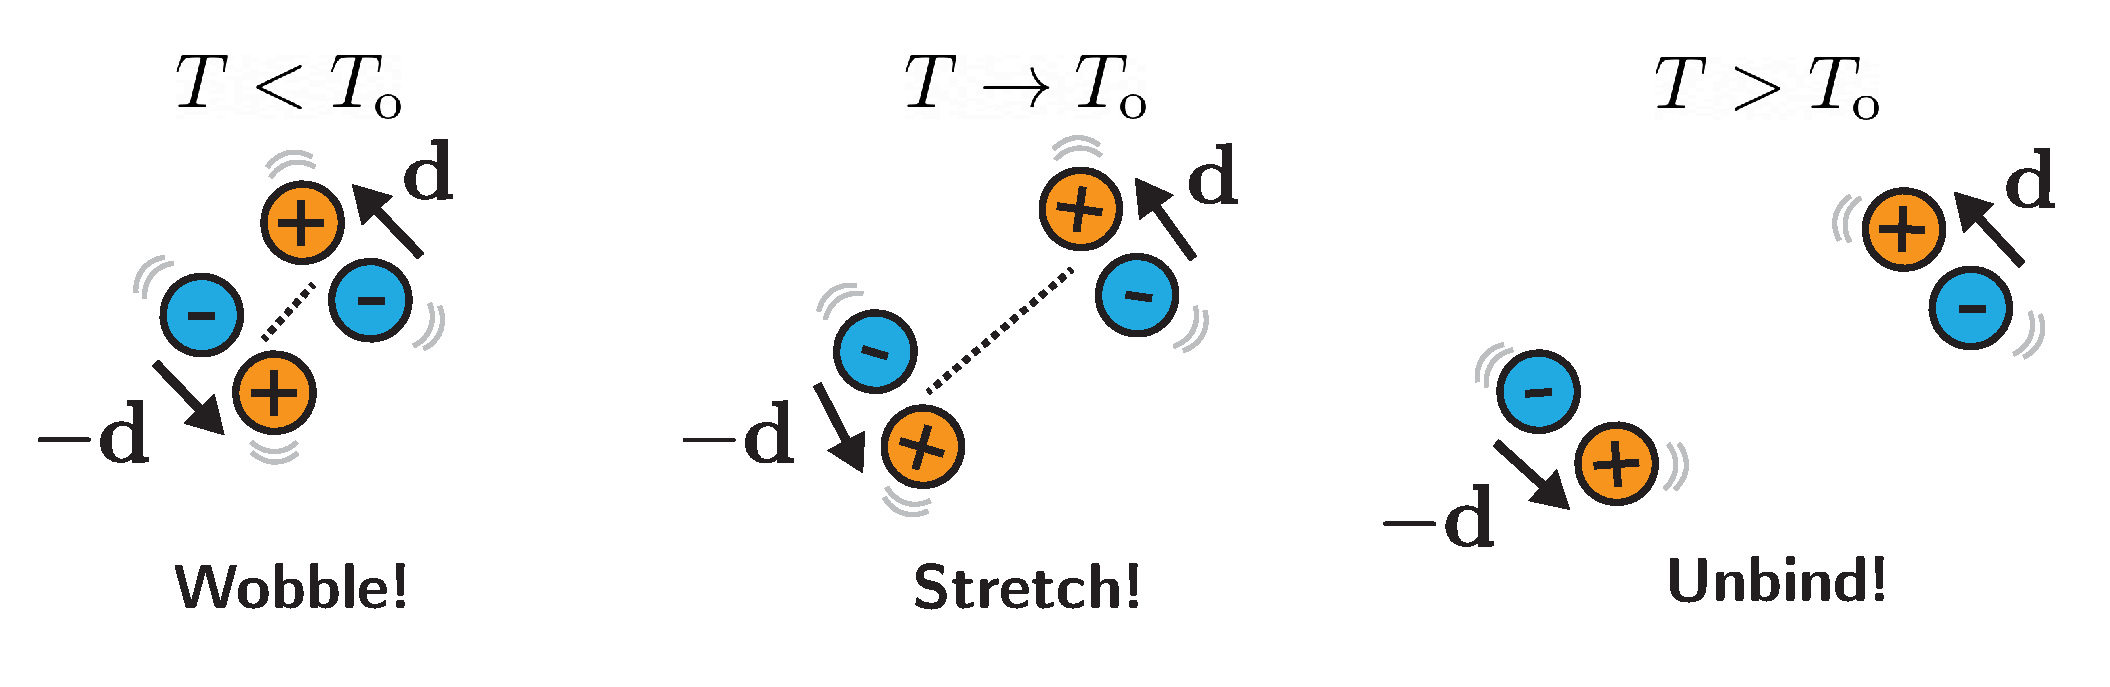
\includegraphics[width=0.85\linewidth]{c.6-kt_energyentropy/dofs_quadrupole-3.pdf}
\end{overprint}
\caption{Dipole-pair configurations and internal modes}
\end{figure}

\end{column}

\begin{column}[T]{0.5\textwidth}

\begin{block}{\centering \large The KT Transition}
Critical binding-unbinding condition
\end{block}

\vspace{0.5em}

$$\boxed{\beta_\mathrm{KT} Y^\mathrm{IS} d_\mathrm{c}^2 = 16 \pi}$$

\vspace{0.5em}

\begin{itemize}
\item \textbf{$T < T_\mathrm{KT}$:} Bound dipole pairs $\to$ solid behavior
\item \textbf{$T > T_\mathrm{KT}$:} Free dipoles $\to$ fluid behavior
\item \textbf{Mechanism:} Entropy drives dipole unbinding
\end{itemize}

\vspace{0.5em}

\begin{block}{\centering Connection to KTHNY Theory}
Similar to Kosterlitz-Thouless-Halperin-Nelson-Young theory of dislocation-mediated melting\footnote{Kosterlitz \& Thouless, \textit{J. Phys. C} (1972-73); Halperin \& Nelson, \textit{PRL} (1978); Nelson \& Halperin, \textit{PRB} (1979); Young, \textit{PRB} (1979)}
\end{block}

\end{column}
\end{columns}

\end{frame}